\begin{frame}
    \begin{figure}
        \hspace*{-320pt}
\includegraphics[width=1.0cm]{vstu_logo}
    \end{figure}
    \vspace{2em}
    \begin{center}
        \large
        \textbf{Методы построения маршрутов общественного транспорта на основе предпочтения жителей}\\
    \end{center}
    \vspace{2em}
    \begin{flushleft}
        \hspace{12em}Автор:~Голубев~А.~В.\\
        \hspace{12em}группа:~САПР-2п1\\
        \hspace{12em}Руководитель:~Щербаков~М.~В.
    \end{flushleft}
    \vspace{3em}
    \centeringВолгоград \the\year\ г.
\end{frame}

% \begin{frame}
%     \frametitle{Актуальность}
%     Изменения в городской среде требуют формирования новых механизмов планирования инфраструктуры города. 
%     Для получения эффективных результатов, следует осуществлять принятие решений на основе актуальных 
%     данных, отражающих предпочтения жителей.
% \end{frame}

\begin{frame}
    \frametitle{Цели и задачи}
    \textbf{Целью} данной работы является разработка метода генерации маршрутов общественного 
    транспорта на основе предпочтений жителей для минимизации дискомфорта перемещения в городе.

    В данной работе рассматриваются к решению следующие задачи:
    \begin{itemize}\itemsep-5pt
        % \item анализ и моделирование предметной области, формирование требований к 
        %     автоматизированной системе;
        % \item проектирование системы: разработка концепции системы, техническое задание и 
        %     разработка проектных решений;
        % \item реализация компонент автоматизированной системы;
        % \item результаты предварительных испытаний автоматизированной системы.
        % ---
        \item генерация псевдореалистичных данных кластеров предпочтений;
        \item разработка метода маршрутизации между кластерами предпочтений;
        \item модификация и использование существующих алгоритмов для задачи маршрутизации;
        \item разработка критериев оценки качества построенных маршрутов;
        \item представление построенных маршрутов на карте;
    \end{itemize}
\end{frame}

\begin{frame}
    \frametitle{Научная новизна}
    \begin{itemize}\itemsep-5pt
        \item \ldots
    \end{itemize}
\end{frame}

% \begin{frame}
%     \frametitle{Методы анализа объекта автоматизации}
%     % Характеристика объекта автоматизации;
%     % Методы применяемые для обследования
%     %% изучение документации;
%     % Подходы функционального моделирования
% \end{frame}

% \begin{frame}
%     \frametitle{Функциональная модель объекта автоматизации}
%     % До 5 слайдов, в зависимости от применяемых моделей
% \end{frame}

% \begin{frame}
%     \frametitle{Требования к системе}
%     % Перечислить требования пользователя у системе
%     %% бизнес-требования
%     %% функциональные
%     %% структурные
% \end{frame}

% \begin{frame}
%     \frametitle{Обоснование необходимости разработки автоматизированной системы}
%     % Обзор аналогов и прототипов
%     %% Список аналогов и прототипов
%     %% Критерии оценки (количественные)
%     % Обосновать необходимость разработки
% \end{frame}

% \begin{frame}
%     \frametitle{Концепции автоматизированной системы}
%     % Альтернативные варианты концепции
%     %% концепция 1 …
%     %% концепция 2 …
%     %% …
%     % Критерии выбора вариантов концепции
%     %% …
%     % Процедура выбора
% \end{frame}

% \begin{frame}
%     \frametitle{Цели и назначение автоматизированной системы}
%     % автоматизировать этап построения маршрутной сети
%     %
%     % Цели разработки автоматизированной системы
%     %% цель 1 (пример сокращение времени, снижение ошибок, )…
%     %% цель 2 …
%     %% …
%     % Назначение АС
%     %% (= главная функция)…

% \end{frame}

% \begin{frame}
%     \frametitle{Требования к структуре автоматизированной системы}
%     % Описать иерархию компонент автоматизированной системы
% \end{frame}

% \begin{frame}
%     \frametitle{Требования к автоматизированным функциям (задачам) системы}
%     % Перечислить (а лучше нарисовать) иерархию автоматизированных функций
% \end{frame}

% \begin{frame}
%     \frametitle{Решения по программному обеспечению}
%     % Отобразить структуру ПО
%     %% UML use case диаграмму 
%     %% UML диаграмму классов 
%     %% Диаграмма деятельности (блок схема)
%     %% Диаграмма развертывания
% \end{frame}

% \begin{frame}
%     \frametitle{Решения по информационному обеспечению}
%     % Структура БД (!?)
% \end{frame}

% \begin{frame}
%     \frametitle{Решения по техническому обеспечению}
%     % Схема автоматизации
% \end{frame}

% \begin{frame}
%     \frametitle{Реализация системы}
%     % календарный график реализации и оценки за программу
%     % перечень документов сформированных в результате
%     % скрин шоты системы автоматизации
% \end{frame}

% \begin{frame}
%     \frametitle{Сценарий испытаний}
%     % Перечислить сценарии из ТЗ в соответствии с которыми проводились 
%     % предварительные испытания и их связь с перечнем  автоматизированных 
%     % функций (слайд 14: требования к автоматизированным функциям...) 
% \end{frame}

% \begin{frame}
%     \frametitle{Результаты предварительных испытаний}
%     % Оценить достижимость цели;
%     % публикации и акт внедрения (или акт проведения предварительных испытаний)
% \end{frame}

\begin{frame}
    \frametitle{Результат}
    \begin{figure}[ht!]
        \centering
        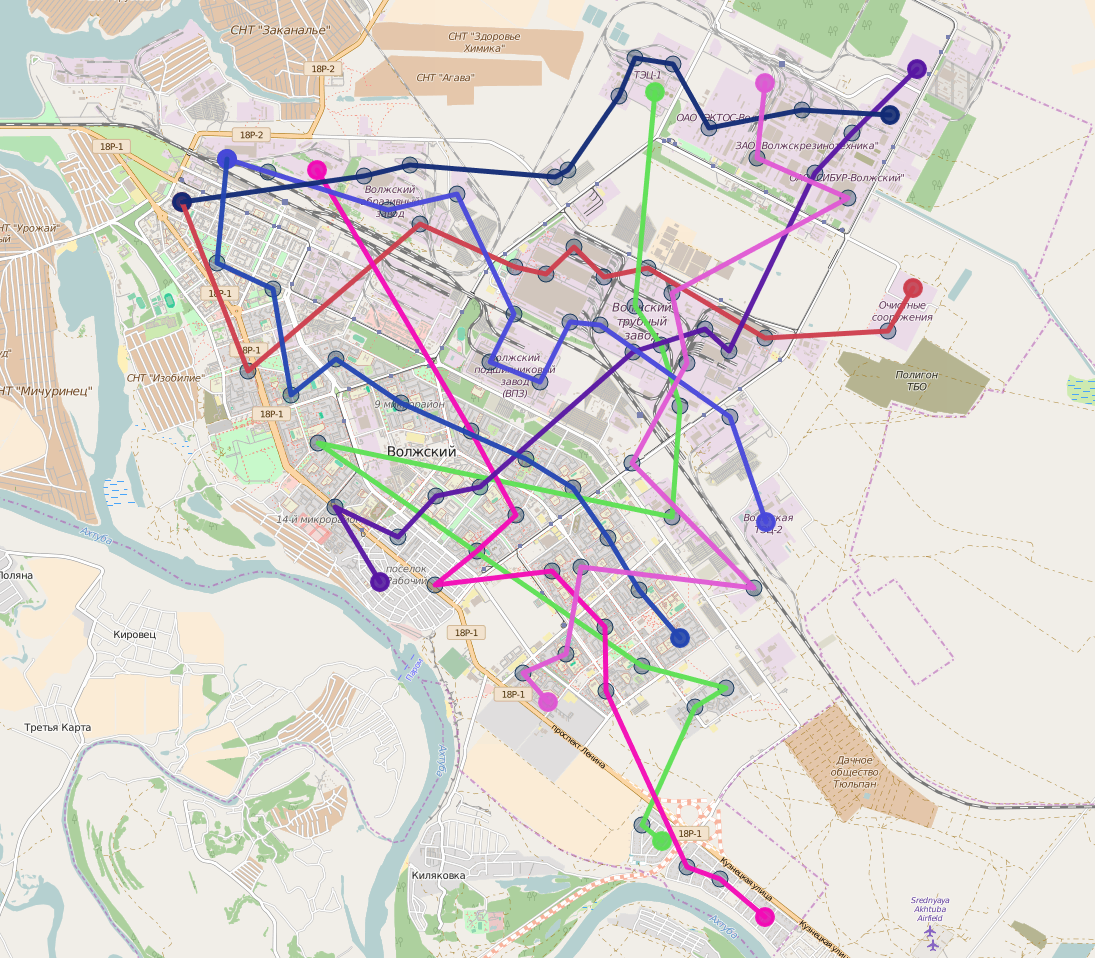
\includegraphics[width=0.8\textwidth]{minimal-01}
    \end{figure}
\end{frame}

\begin{frame}
    \frametitle{Результат}
    \begin{figure}[ht!]
        \centering
        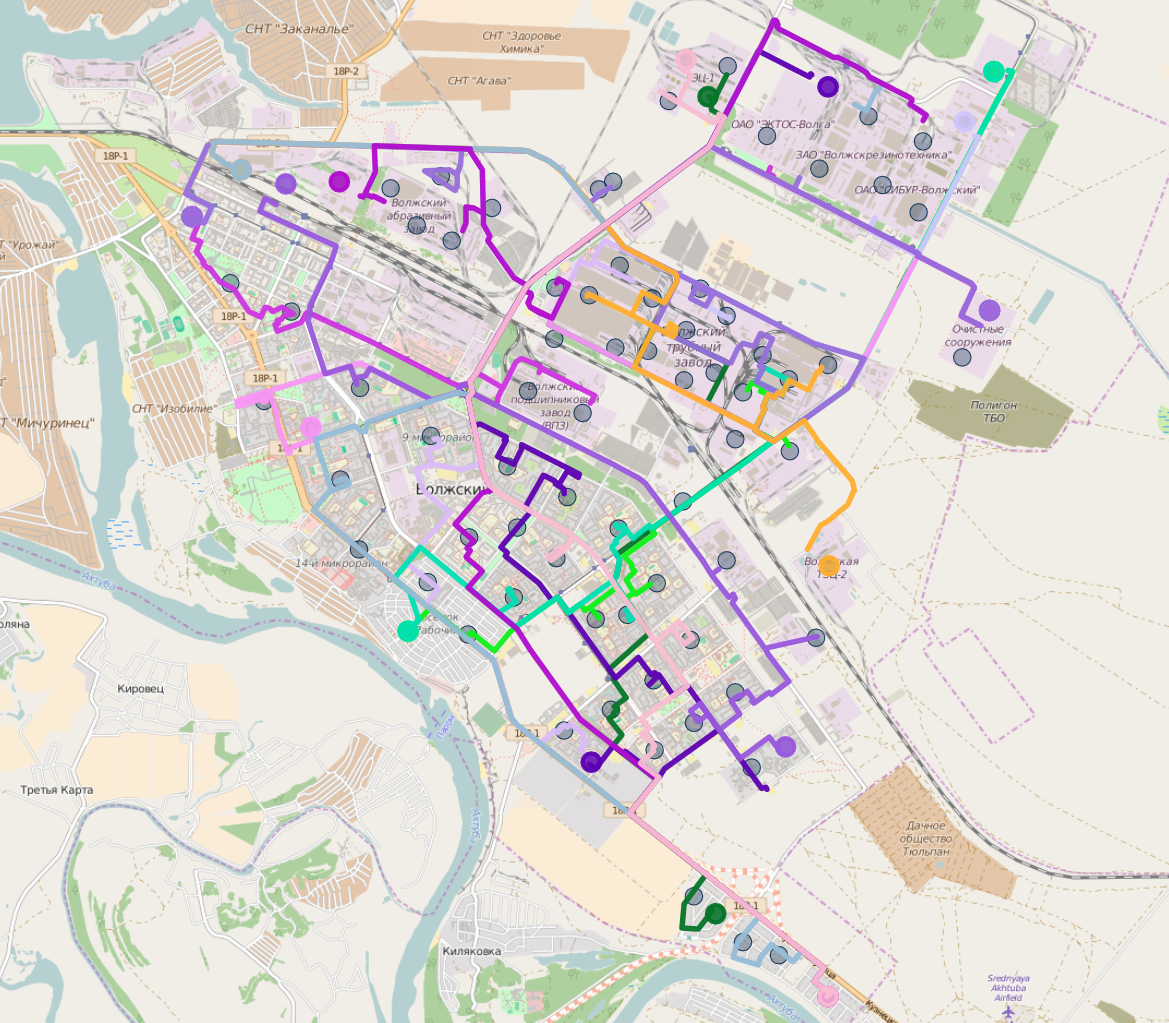
\includegraphics[width=0.7\textwidth]{minimal-02}
    \end{figure}
    \url{http://vstu-cad-stuff.github.io/routing/geojson/}
\end{frame}

\begin{frame}
    \frametitle{Публикации}
    \scriptsize
    \begin{thebibliography}{10}
        \bibitem{first} Golubev A, Chechetkin I, Solnushkin K.S., Sadovnikova N., Parygin D., Shcherbakov M., 
            Brebels A., Strategway: web solutions for building public transportation routes using big geodata 
            analysis // Proceedings of The 17th International Conference on Information Integration and 
            Web-based Applications \& Services (iiWAS2015) (December 11 - 13, 2015 Brussels, Belgium) 
            ACM New York, New York pp. 665 - 668
        \bibitem{second} Садовникова Н.П., Щербаков М.В., Парыгин Д.С., Солнушкин К.С., Голубев А.В., 
            Чечёткин И.А. Комплекс инструментов интеллектуального анализа данных strategway для поддержки 
            принятия решений по управлению развитием инфраструктуры города / В сборнике: Развитие средних 
            городов: замысел, модели, практика Материалы III Международной научно-практической конференции. Волгоград, 2015. С. 147-150
        \bibitem{third} М.В. Щербаков, Н.П. Садовникова, Д.С. Парыгин, А.В. Голубев, И.А. Чечеткин 
            Автоматизация поддержки принятия решений по разработке маршрутов общественного транспорта на 
            основе анализа данных о корреспонденциях жителей // Вестник компьютерных и информационных 
            технологий (сдана в редакцию)
    \end{thebibliography}
\end{frame}

\begin{frame}
    \frametitle{Вопросы}
    \begin{itemize}
        \item Голубев Алексей Владимирович
        \item \href{mailto:ax.golubev@gmail.com}{ax.golubev@gmail.com}
    \end{itemize}
\end{frame}